\section{Results \& Verification}
\label{sec:results}
% read revit file and 

\subsection*{Input Data and Experiment setting}
The Input Data will be BIM model in Revit format, which is a hospital. We assume that the renovation activity is to install 
a new air conditioning system in the hospital. Here is the BIM model of the hospital (Figure \ref{fig:hospital}).
\begin{figure}
    \centering
    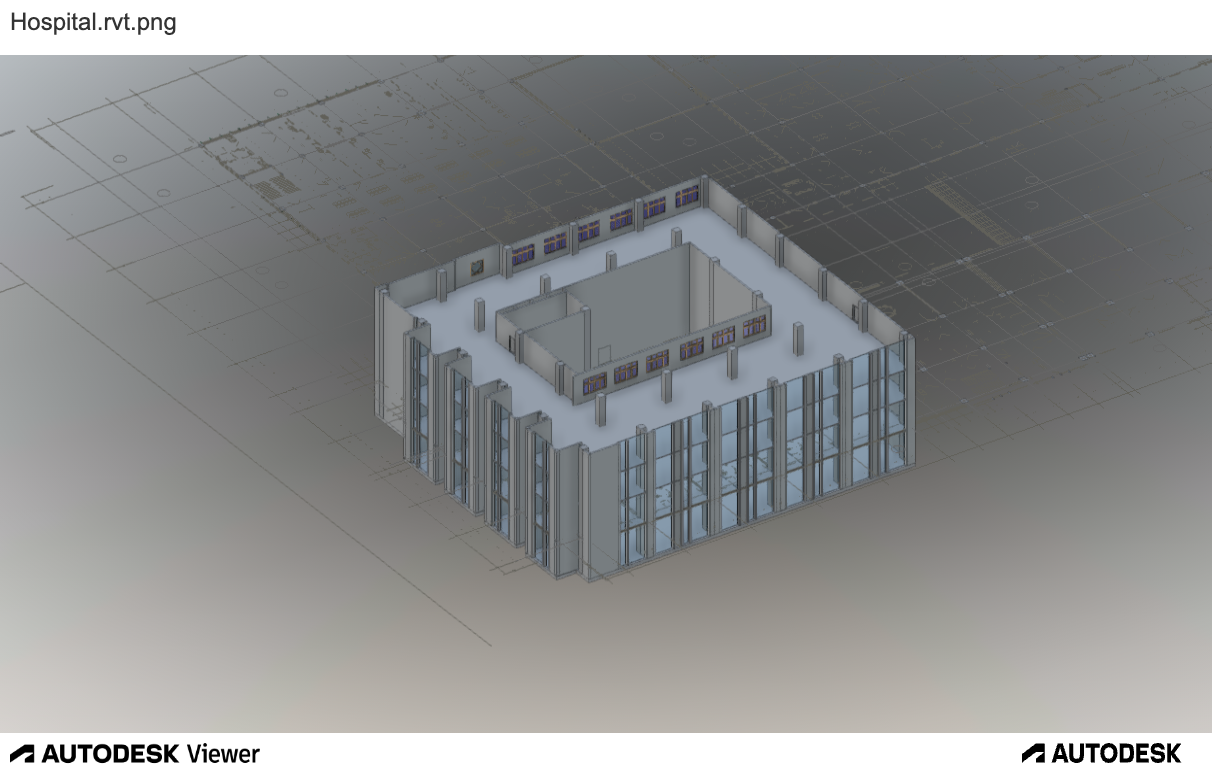
\includegraphics[width=0.5\textwidth]{figures/Hospital.rvt.png}
    \caption{Hospital BIM model}
    \label{fig:hospital}
\end{figure}

The LLM model we choose is OpenAI's GPT-4o. We call the API of GPT-4o in Python environment to build our safety management system.
The platform of Graph Database we choose is Neo4j. We use the Neo4j Desktop to build the graph database and query the graph database.

\subsection{Graph Database Construction}
The first step is converting the ontology to the graph database. The detailed steps is shown in section \ref{sec:ontology_coarse}
Here we should the overview graph of ontology stored in Neo4j (Figure \ref{fig:ontology_graph}).
\begin{figure}
    \centering
    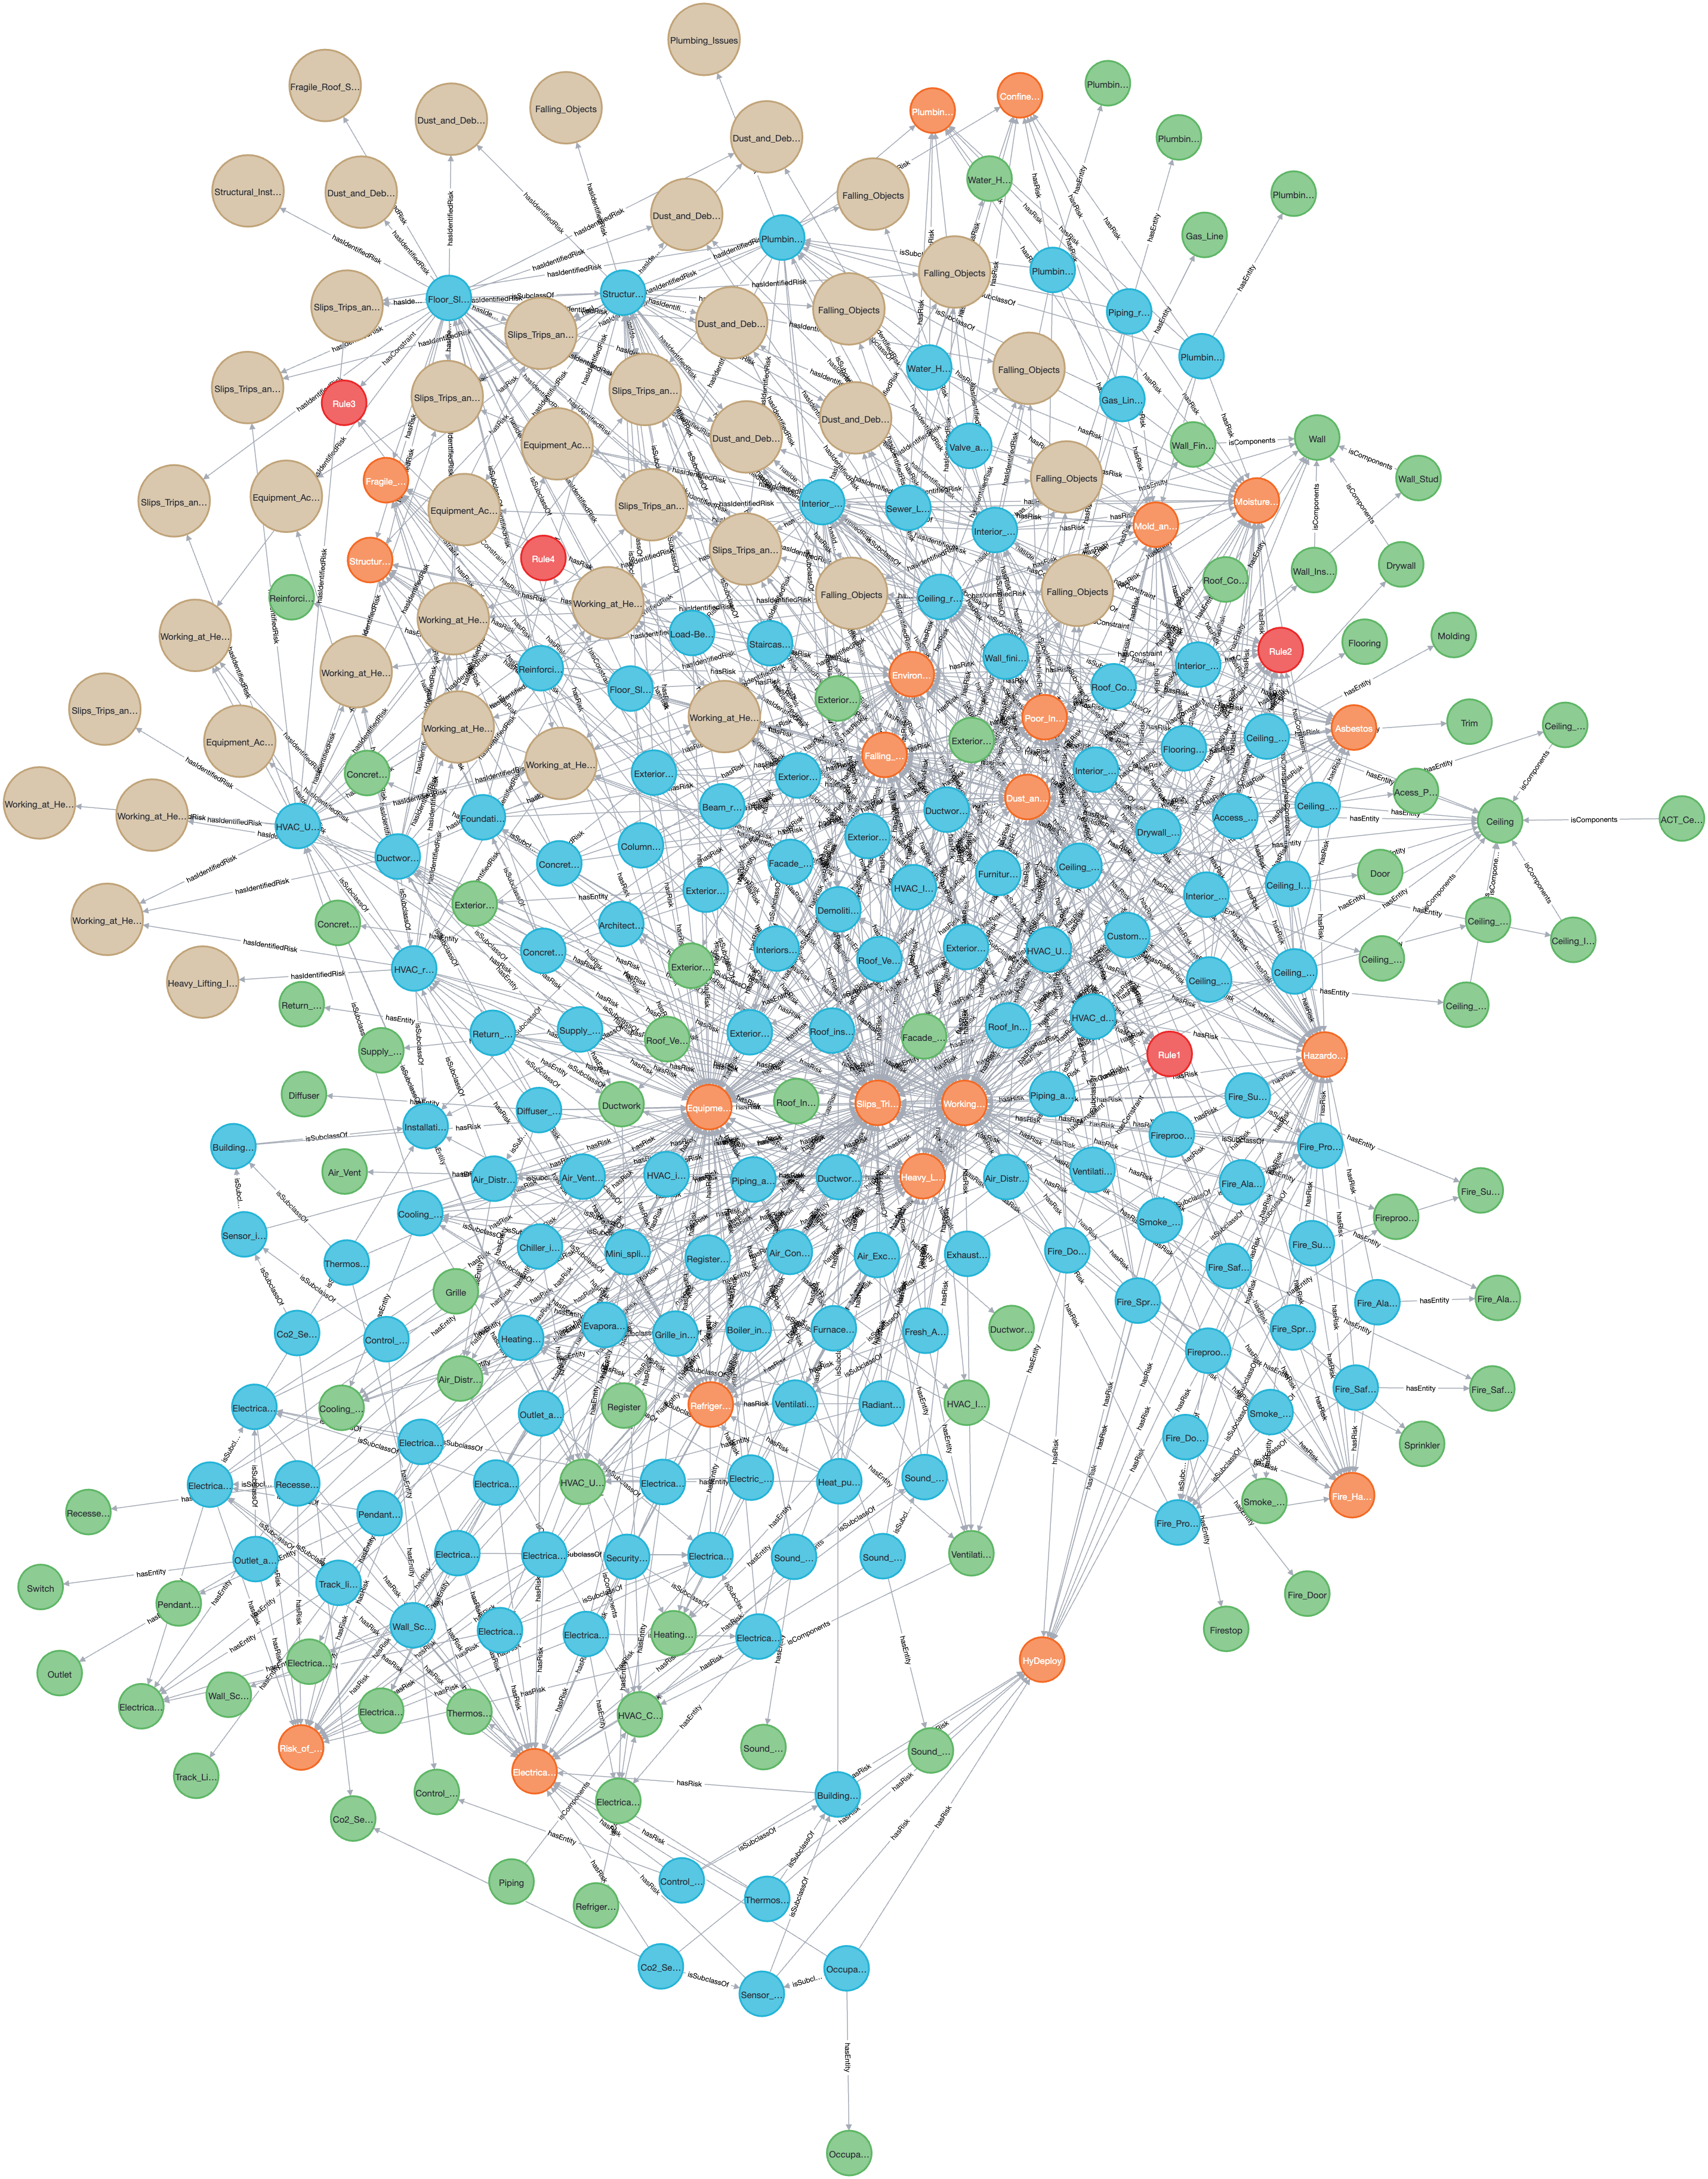
\includegraphics[width=0.5\textwidth]{figures/graph (2).png}
    \caption{Ontology Graph in Neo4j}
    \label{fig:ontology_graph}
\end{figure}
\subsection*{Ontology Enrichment}
We input the images and regulation documents to the LLM model. The LLM model will generate two more relations on original ontology. \\
The first relation is the relation between the renovation activities and the risks.
 There is a new relation called 'hasIdentifiedRisk' between renovation activities and identified risk from collected images on each activited during the renovation process. 
 The same risk may appeared more than once among different images, we will calculate the frequency of each risk appeared in the images. The frequency of each identifed risk will be stored in the attribute of the risk node in graph. 
 
 The second relation is the regulation related to renovation activities. The LLM model will generate a new relation called 'hasRelatedRegulation' between renovation activities and the regulation documents.
 This relation indicates that the regulation is applicable to the renovation activities. Another relation LLM extracted from regulation document is 
 the relation "hasRegulatedEntity", which is relation between activities and entities appeared in the regulation document,
 which indicates that the entities in renovation activities has to be regulated by the regulation document.

\begin{figure}
    \centering
    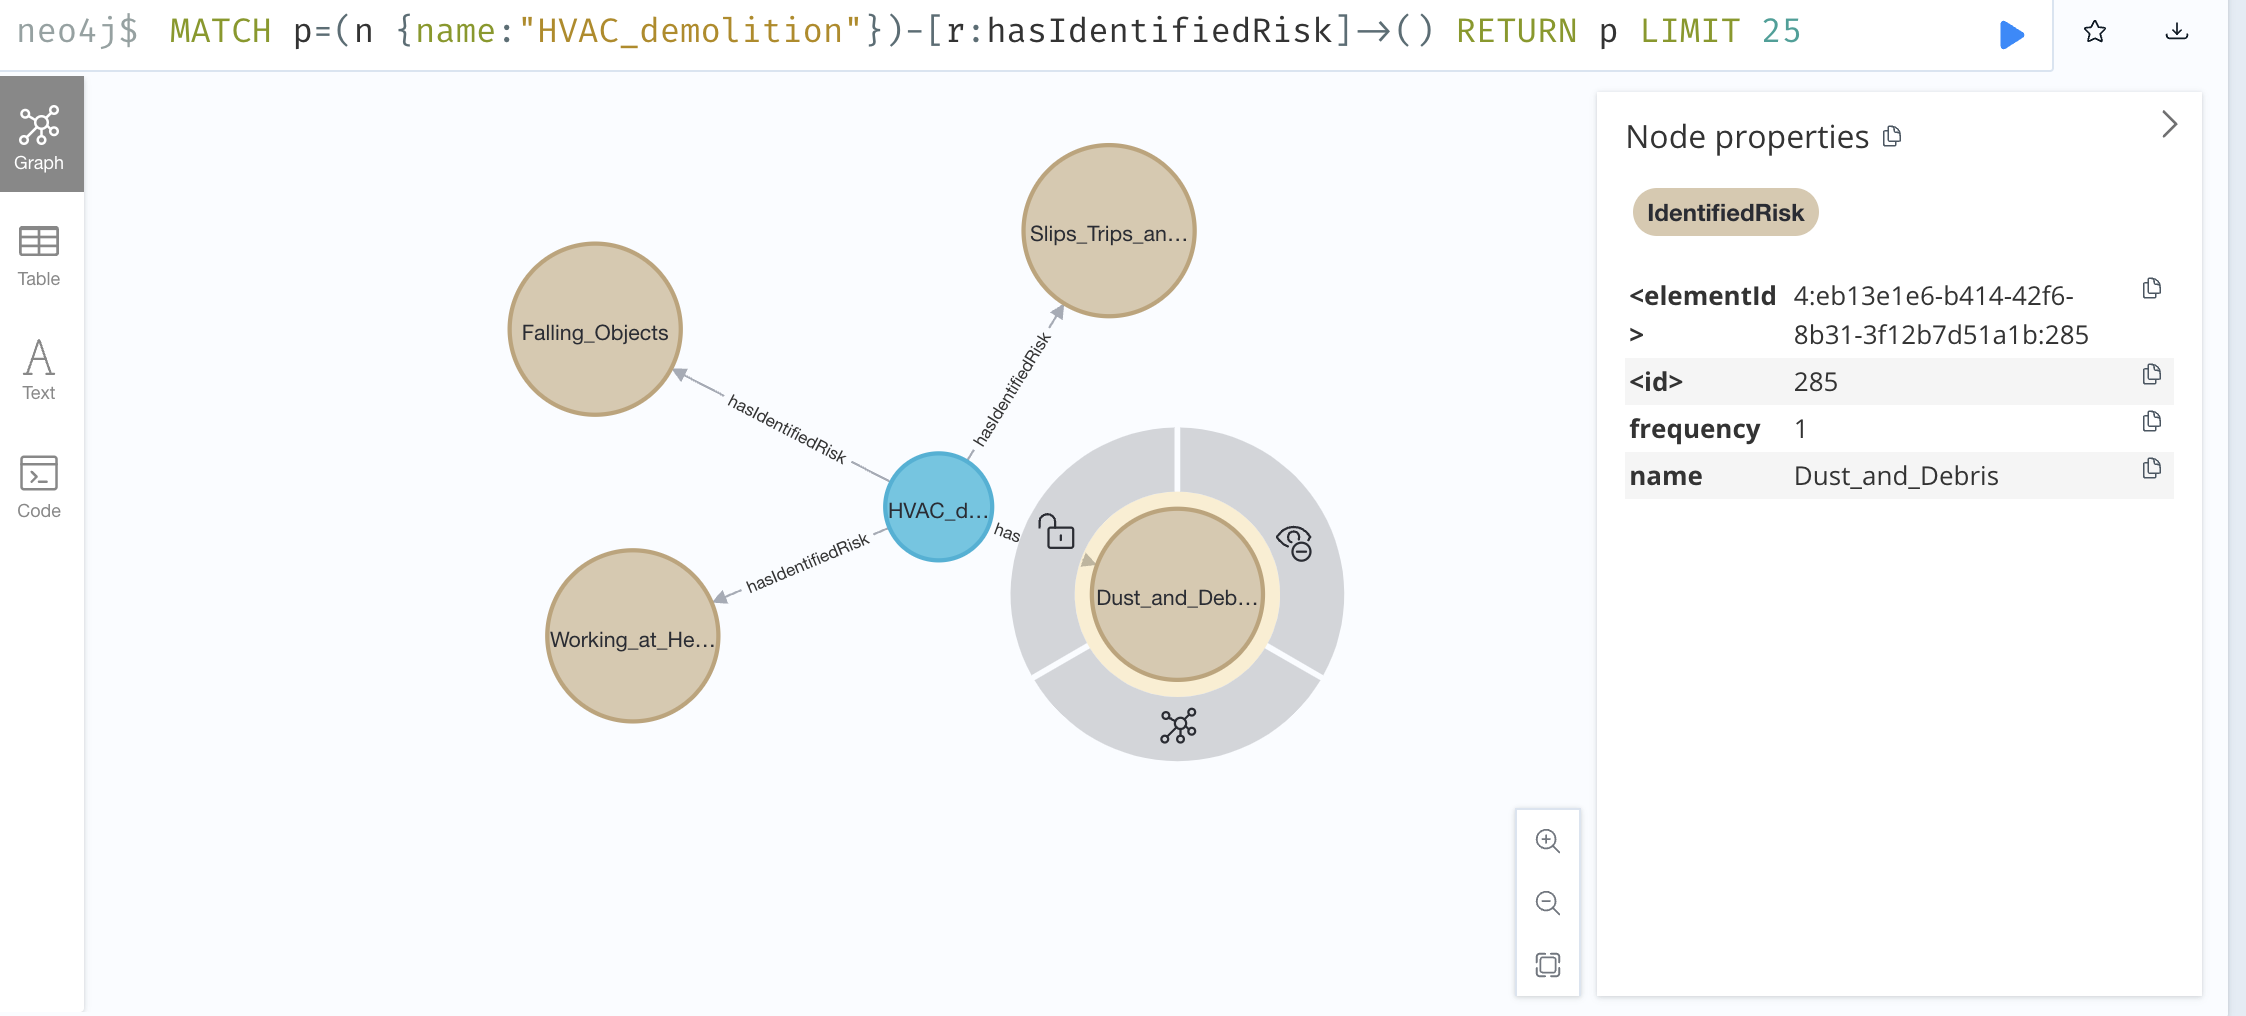
\includegraphics[width=0.5\textwidth]{figures/risk identified.png}
    \caption{Samples of extracted relation from images in Neo4j}
    \label{fig:image_enrichment}
\end{figure}
\begin{figure}
    \centering
    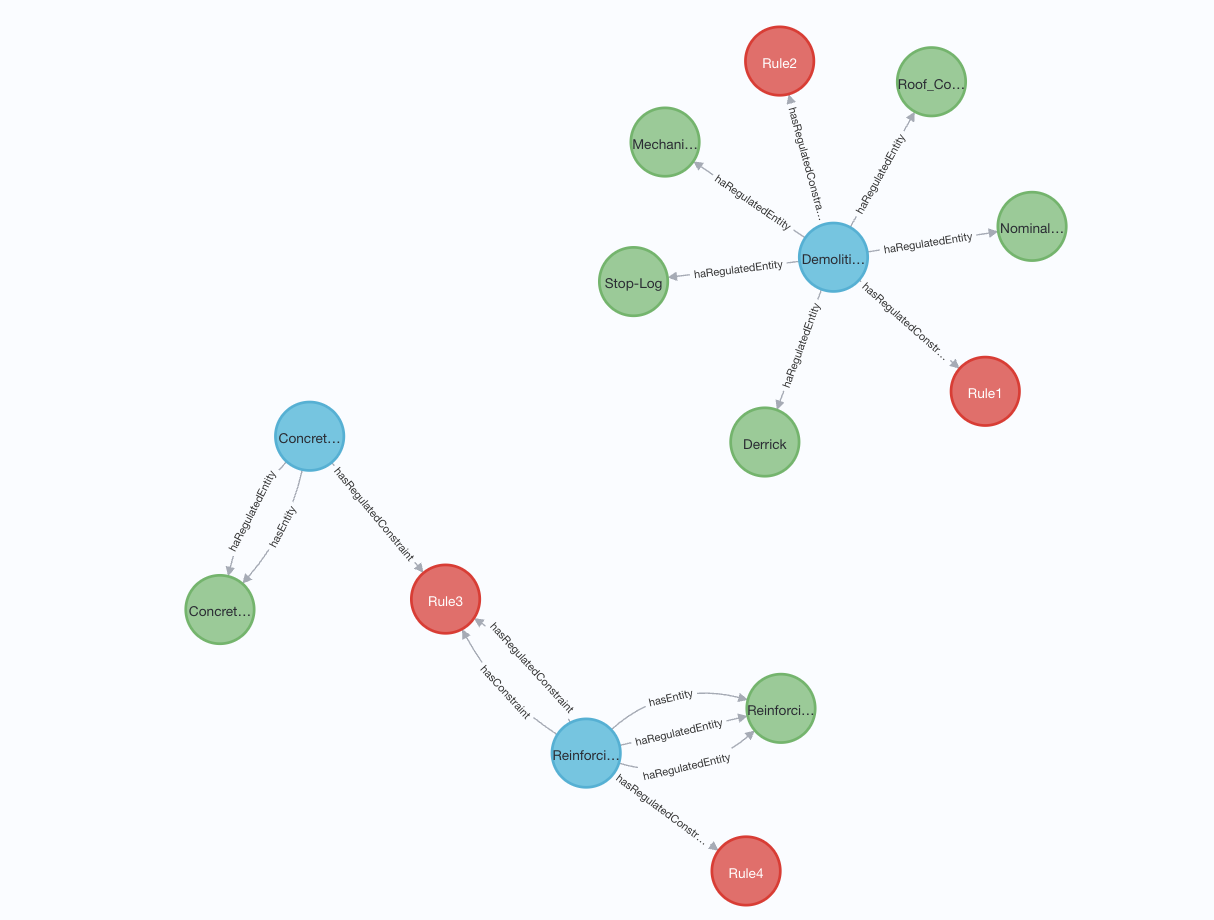
\includegraphics[width=0.5\textwidth]{figures/regulation.png}
    \caption{Samples of extracted relation from regulation documents Neo4j}
    \label{fig:ontology_graph_enriched}
\end{figure}

After the ontology enrichment, the ontology graph in Neo4j is shown in Figure \ref{fig:ontology_graph_enriched}, \ref{fig:image_enrichment}.
The extracted information can be easily queried from the graph database, given the name of renovation activities involved in the renovation process.

\subsection{The Final Interactive Interface}
The final interactive interface is a QA system, which is run on command line mode. It could be transfer to a web-based platform
or Autodest Revit. But for the convenience of the experiment, we only implement the command line mode.

% the result of the system is still undefine,
The dialogue between the user and the system is shown in the Figure \ref{fig:dialogue}.
\begin{figure}
    \centering
    \label{fig:dialogue}
    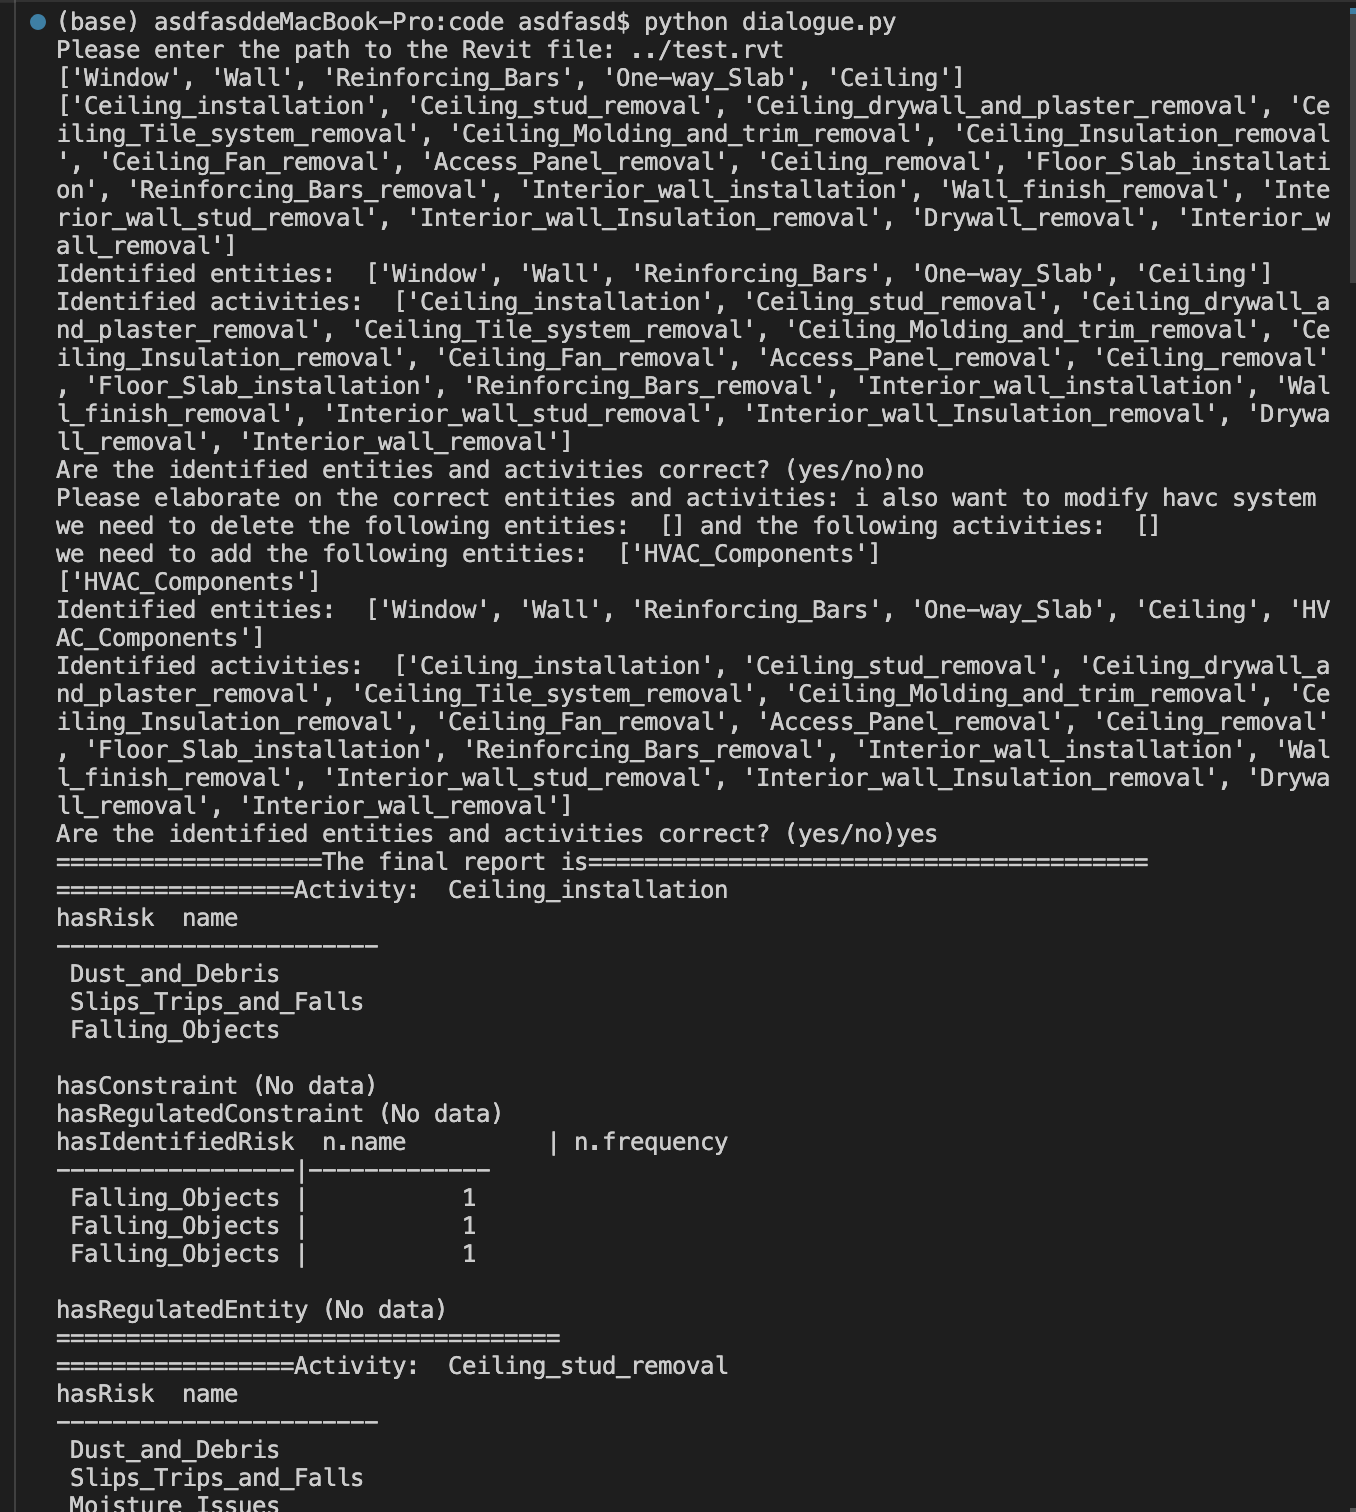
\includegraphics[width=0.5\textwidth]{figures/output screen shot.png}
    \caption{Dialogue between the user and the system}
    
\end{figure}

As we shown in the dialogue screen shot, firstly, the use input the direcotry of the BIM model in Revit format. 
Then the system will load the BIM model and extract the building components in the model and searching the related renovation activities from 
the ontology graph. Then user can input their requirements such as the renovation plan they hoep to implement, then the system will
modify the list of possible renovation activities and entities. Finally, the report of the renovation activities, risks, and related regulations will be generated.

Sample of results shown in the Table  \ref{tab:input_output}.
\begin{table}
    \centering
    
    \label{tab:input_output}
    \begin{tabularx}{0.5\textwidth}{|c|X|X|X|}
        \hline
        Step & Input & Output &  Results \\
        \hline
        1 & Directory of BIM & Automatical search for all activities related to the building components: & see appendix  \ref{fig:output1}, \ref{fig:output1.1}\\
        \hline
        2 & I only want to install an air conditioner on the wall & The possible activities according to user description & see appendix \ref{fig:output2}, \ref{fig:output1.2}\\
        \hline
        3 & Agree with it & Generated report & see appendix \ref{fig:output3}, \ref{fig:output1.3} \\
        \hline
    \end{tabularx}
    \caption{Sample of input and output in each step}
\end{table}

\subsection*{Summary}
In summary, our system can adaptively query the related activites, risks, and regulations from the ontology graph based on the user's input.
Compared with previous onotlogy-based safety management system for renovation activitis \cite[]{doukari2024ontology},
our query result not only contains more knowledge, which is extracted from multimodal data, but also the searching result is more comprehensive,
because the LLM system will automatically search all possible activities and entities related to the user's input.

However, we should also notice that, the dialogue format is rigid and many missing data are found in the results. 
Because we have not fine-tuned the LLM, currently the QA system require user answer in a specific format, which is flexible and robust.
The missing data in the results is due to the lack of data support, which may lead to inaccurate ontology and unreliable results.   
Since this paper only demonstrates the feasibility of the system, the future work will focus on the fine-tuning of the LLM model and the data collection to improve the performance of the system.






